\section{MCMC Hammer (linear model)}

For this problem, we are going to fit the data with the same model described by equation \ref{eq:linearModel}. For this case, we are going to use the MCMC Hammer method. This method is being implemented by doing the following:
\begin{itemize}
    \item From the best fit parameters generates N randomly generated initial guesses using a normal distribution or multivariate normal distribution for more than one parameter. These are called the walkers.In python, it will be an array of different values where each row will have length equal to the number of parameters.
    \item Called the emcee.EnsembleSampler() specifying the logarithm of $\pi$ given by equation \ref{eq:piMCMC} as the posterior probability for normal distributed parameters.
    \item Then, we run the sampler by doing \\ sampler.run\_mcmc(walkersArray,No.trials). \\
    For this step the trial number can be relatively small just to go through the burn-in period.
    \item We reset the sampler and run it again but this time using the output positions from the last step as the walkers Array and a large number of trials.
\end{itemize}

To adjust the number of trials for the burn-in period we can analyze the posterior probability and see if there are values
The last step will mapped the posterior probability of all the parameters. 
Figure \ref{fig:linearEmcee} shows the posterior probability for the parameters using a linear model.

Note that this posterior probability resembles the one shown in Figure \ref{fig:LinearHastings} as expected since we are using the same data and model. 
The mean values are slightly different but are still within the error range of each other. 

% Repeat problem 5.6 using either the
% emcee package or by implementing your own slide-step sampler in place of the M-H sampler.
% Make sure you clearly describe both your implementation as well as what checks you do to
% make sure that things have worked well.

\begin{figure}
    \centering
    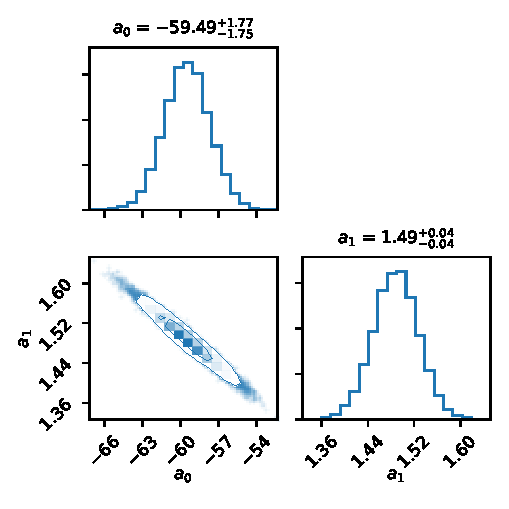
\includegraphics{CodeAndFigures/LinearModelEmcee.pdf}
    \caption{The posterior probability of the parameters of the linear model described by equation \ref{eq:linearModel} sampled by using MCMC Hammer (emcee) Method. The contours show the 68.3\% and 95\% confidence intervals.}
    \label{fig:linearEmcee}
\end{figure}

